
\chapter{La mise en \oe{}uvre de l'API}
\label{implementation.chap}

\subsection{Parall\'elisation}

La cr\'eation du code parall\`ele a \'et\'e le domaine des experts. La complexit\'e du code parall\`ele diminue la productivit\'e, ce qui peut augmenter les co\^uts de d\'eveloppement. \TT{PpFf} permet aux programmeurs de composer du code s\'equentiel et de l'ex\'ecuter en parall\`ele. Dans une interface unique, l'\TT{API} offre deux mod\`eles de parall\'elisme : le parall\'elisme de flux et \TT{Task-Farm}.


\subsubsection{Parall\'elisme de flux}

Le parall\'elisme de flux consiste \`a ex\'ecuter plusieurs \'etapes d'un traitement s\'equentiel en parall\`ele en leur faisant traiter des données diff\`erentes. Les donn\'ees se succ\`edent ainsi les unes aux autres dans les diff\'erentes \'etapes, nomm\'ees aussi des stages. Le traitement effectu\'e dans un stage \`a un instant donn\'e peut d\'ependre des traitements effectu\'es par ce stage pour les donn\'ees pr\'ec\'edentes. Ce fonctionnement permet de parall\'eliser des traitements avec de fortes d\'ependances entre les donn\'ees sans avoir recours \`a de nombreuses synchronisations. 
Un flux avec n stages peut \^etre formellement exprim\'e sous la forme d'une composition s\'equentielle d'op\'erateurs sur les \'el\'ements d'entr\'ee. 

\[
	O(x) = O_n( \ldots (O_k( \ldots O_1(x)) \ldots ) \ldots ));
\]

Dans ce cas, la parall\'elisation est repr\'esent\'ee par un graphique lin\'eaire de n travailleurs. Chaque travailleur correspond \`a une op\'eration sp\'ecifique. La figure~\ref{ParallelismeDuFlux.fig} montre la repr\'esentation graphique du parall\'elisme de flux. Cette solution n'acc\'el\`ere pas le calcul d'un seul \'el\'ement. Par contre, elle am\'eliore le d\'ebit de sortie.

\begin{figure}[ht]
\centering
     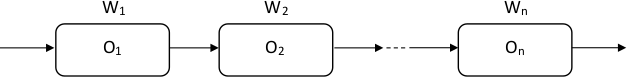
\includegraphics[width=1.0\textwidth]{Figures/ParallelismeDuFlux.jpg}
      \caption{Le parall\'elisme de flux.}
       \label{ParallelismeDuFlux.fig}
\end{figure}



\subsection{Stages}

Le traitement du flux de donn\'ees est mod\'elis\'e en utilisant une cha\^{\i}ne d'\'etapes. Dans notre API, une \'etape est repr\'esent\'ee par un \texttt{Stage}, et chaque \texttt{Stage} est compos\'e d'un ou plusieurs op\'erateurs. Notons toutefois que ce module n'est pas visible \`a l'utilisateur. 


\GT{Donc, en lien avec ma remarque pr\'esent\'ee plus haut: si la
notion de Stage n'est pas visible \`a l'utilisateur, elle ne devrait
donc pas faire partie de la pr\'esentation de l'API. Elle devrait
plut\^ot \^etre trait\'ee dans la partie Mise en \oe{}uvre
(impl\'ementation).}
